\documentclass[a4paper]{article}

\usepackage[english]{babel}
\usepackage[utf8x]{inputenc}
\usepackage{amsmath, amssymb}
\usepackage{color}
\usepackage{tikz}
\usepackage{tkz-graph}
\usetikzlibrary{arrows,petri,topaths,shapes,positioning}
\usepackage[colorinlistoftodos]{todonotes}
\usepackage{multicol}

%-----------------------------------%

%%%%%%%%%%%%%%%%%%%%%%%%%%%%%%%%%%%
%                                 %
% Vertex, Edge, and Weight Styles %
%                                 %
%%%%%%%%%%%%%%%%%%%%%%%%%%%%%%%%%%%
% vertex styles
\tikzstyle{vertex}=[circle,fill=black!20,minimum size=20pt,inner sep=0pt]
\tikzstyle{selected vertex} = [vertex, fill=blue!40]
\tikzstyle{possible vertex} = [vertex, fill=green!40]
\tikzstyle{bad vertex}=[circle,fill=red!40,minimum size=20pt,inner sep=0pt]
\tikzstyle{Euler vertex}=[circle,fill=black!100,minimum size=5pt,inner sep=0pt]

% edge styles
\tikzstyle{edge} = [draw,thick,-]
\tikzstyle{selected edge} = [draw,line width=5pt,-,blue!50]
\tikzstyle{possible edge} = [draw,line width=5pt,-,green!50]
\tikzstyle{bad edge} = [draw,line width=5pt,-,red!50]

% weight styles
\tikzstyle{weight} = [font=\small]

%-----------------------------------%

% Declare layers
\pgfdeclarelayer{background}
\pgfsetlayers{background,main}

%-----------------------------------%


\title{MATH 101 - Handout 1}

\begin{document}

\section*{MATH 101 - Handout 1}

\section{Graph Theory}

\subsection{Terminology}

\begin{multicols}{3}
\begin{itemize}

\item Graph
\item Vertex
\item Edge
\item Adjacent Vertices
\item Degree (Valence)
\item (Dis-)Connected
\item Path
\item Circuit
\item Euler Path
\item Euler Circuit
\item Euler's Theorem
\item Eulerization
\item Best Eulerization
\item Semi-Eulerization
\item Hamilton'n Circuit
\item Nearest Nbr Alg'm
\item Cheap Link Alg'm
\item Brute-force Alg'm
\item Tree
\item Spanning Tree
\item Kruskal's Alg'm

\end{itemize}
\end{multicols}

\subsection{Exercises}

%
% Make a Network
%
\begin{figure}[h]
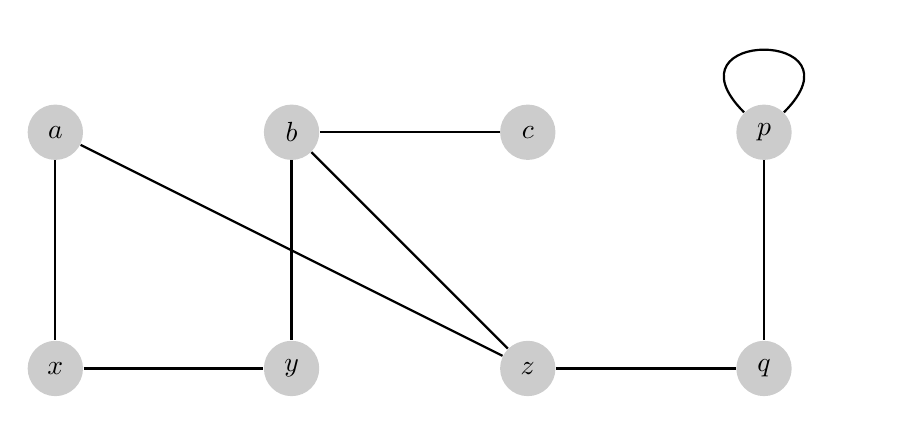
\begin{tikzpicture}[scale=3.0, auto,swap]

% First we draw the vertices
\foreach \pos / \name in {{(-1,1)/a},{(0,1)/b},{(1,1)/c},{(-1,0)/x},{(0,0)/y},{(1,0)/z},{(2,1)/p},{(2,0)/q}}
\node[vertex] (\name) at \pos {$\name$};

% Connect vertices with edges and draw weights
\foreach \source/ \dest in {a/x,a/z,x/y,b/y,b/c,b/z,p/q,z/q}
\path[edge] (\source) -- (\dest);

\Loop[dist=0.5cm,dir=NO,style={thick},label=$ $,labelstyle=below](p)

\end{tikzpicture}
\end{figure}

\begin{enumerate}
\item What are the vertices of the graph?
\item What are the edges of the graph?
\item What are the degrees of each vertex:
\begin{multicols}{2}
\begin{itemize}
\item $\deg(a)=?$
\item $\deg(b)=?$
\item $\deg(c)=?$
\item $\deg(x)=?$
\item $\deg(y)=?$
\item $\deg(z)=?$
\item $\deg(p)=?$
\item $\deg(q)=?$
\end{itemize}
\end{multicols}
\end{enumerate}

\end{document}
